\documentclass[a4paper]{article}
\usepackage[utf8]{inputenc}
\usepackage[T1]{fontenc}
\usepackage[francais]{babel}
\usepackage[top=2cm, bottom=2cm, left=2cm, right=2cm]{geometry}
\usepackage{amsthm}
\usepackage{amsmath}
\usepackage{amssymb}
\usepackage{mathrsfs}
\usepackage{multirow}
\usepackage{graphicx}
\usepackage{float}
\floatplacement{figure}{ht}
\title{Questions de théorie pour l'examen oral de physique 3 : proposition de réponses}
\date{Classe de 6BE, 18 juin 2013}
\author{}
\begin{document}
\maketitle
\section{Les ondes}
\subsection{Énoncé}
\paragraph{}\textbf{Propagation d'une onde dans un milieu à une dimension : équation générale, réflexion sur une extrémité libre ou fixe. Ondes stationnaires résonnantes sur une corde ou dans un tuyau : posistionsdes nœuds et des ventres de déplacement (et de pression dans le cas des ondes acoustiques).}
\subsection{Équation d'une onde}
L'équation d'une onde s'écrit de la manière suivante :
\[y(t,x)=Rsin\left(2\pi\left(\frac{t}{T}-\frac{x}{\lambda}\right)+\varphi\right)\]
\paragraph{}Cette formule peut se déduire de celle de l'oscillateur harmonique :
\[y(t)=Rsin(\omega t+\varphi)\]
\paragraph{}Cependant, il serait intéressant d'exprimer ceci en fonction de $x$ en plus de $t$. À cette fin, nous partons du fait que considérer l'onde au point $0$ à l'instant $t$ reviens au même que de considérer l'onde au point $x$ à l'instant $t+\frac{x}{c}$. En effet, vu que l'onde se déplace à la vitesse $c$, il lui faudra un temps $\frac{x}{c}$ pour parcourir la distance supplémentaire.
\paragraph{}Remplaçons donc $t$ par $t+\frac{x}{c}$ dans l'équation de l'onde.
\[y(t,x)=Rsin\left(\omega \left(t+\frac{x}{c}\right)+\varphi\right)\]
\paragraph{}Vu que $\omega=\frac{2\pi}{T}$ alors
\[y(t,x)=Rsin\left(\frac{2\pi}{T} \left(t+\frac{x}{c}\right)+\varphi\right)\]
\[=Rsin\left(2\pi \left(\frac{t}{T}+\frac{x}{cT}\right)+\varphi\right)\]
\paragraph{}Vu que $T$ est la période temporelle, si nous la multiplions par la vitesse $c$, nous obtenons $cT$ qui est la période spatiale, aussi appelée longueur d'onde $\lambda$. Donc en substituant $\lambda$ à $cT$, nous obtenons
\[y(t,x)=Rsin\left(2\pi \left(\frac{t}{T}+\frac{x}{\lambda}\right)+\varphi\right)\]
\paragraph{}Cette équation est bien celle présentée ci-dessus.
\subsection{Réflexion d'une onde}
\subsubsection{Sur une extrémité fixe}
\paragraph{}Lorsqu'une onde se réflechit sur une extrémité fixe, elle se réflechit mais elle s'inverse (voir dessin)
\begin{figure}
\begin{center}
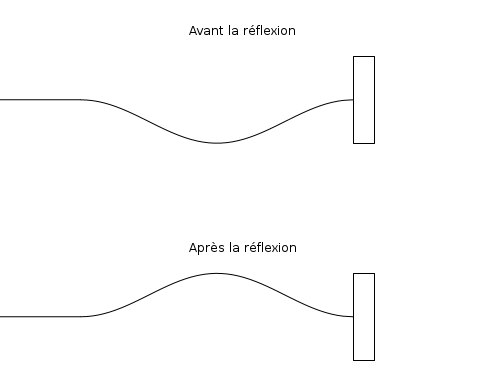
\includegraphics[width=5cm]{imgs/reflfixe.png}
\end{center}
\caption{Réflexion d'une onde sur une extrémité fixe}
\label{Réflexion d'une onde sur une extrémité fixe}
\end{figure}
\subsubsection{Sur une extrémité libre}
\paragraph{}Lorsqu'une onde se réflechit sur une extrémité fixe, elle se réflechit à l'identique (voir dessin)
\begin{figure}
\begin{center}
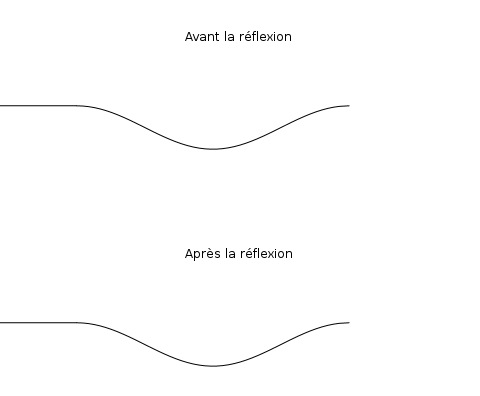
\includegraphics[width=5cm]{imgs/refllibre.png}
\end{center}
\caption{Réflexion d'une onde sur une extrémité libre}
\label{Réflexion d'une onde sur une extrémité libre}
\end{figure}
\subsection{Les ondes stationnaires}
\paragraph{}Une onde stationnaire est une onde «qui n'avance pas» c'est à dire dont les extrema et les points d'inflexion restent fixes dans l'espace. Il est possible d'en produire grâce à la réflexion d'une onde dans un tuyau ou dans une corde.
\subsubsection{Équation de l'onde réfléchie}
\paragraph{}Calculons la fonction de l'onde réfléchie. Elle est obtenue à partir de celle de l'onde incidente. Il faut modifier la variable $x$, en effet l'onde réfléchie n'a pas parcouru un distance $x$ pour arriver à ce point : Elle a du en effet, parcourir le tuyau ou la corde de longueur $L$ avant de se réfléchir et de parcourir une distance $L-x$ pour arriver au point $x$. Donc il faut remplacer $x$ par $2L-x$ dans l'équation de l'onde incidente pour obtenir celle de l'équation de l'onde réfléchie. C'est-à-dire :  
\[y_{incidente}(t,x)=Rsin\left(2\pi \left(\frac{t}{T}+\frac{x}{\lambda}\right)+\varphi\right)\]
\[y_{r\acute{e}fl\acute{e}chie}(t,x)=y_{incidente}(t,2L-x)=Rsin\left(2\pi \left(\frac{t}{T}+\frac{2L-x}{\lambda}\right)+\varphi\right)\]
\subsubsection{Onde résultante de la réflexion d'une onde sur une extrémité fixe.}
\paragraph{}Pour calculer cette onde résultante, nous devons additionner l'onde incidente à l'onde réfléchie en n'oubliant pas d'inverser le signe de l'onde réfléchie vu que l'extrémité est fixe.
\[y_{r\acute{e}sultante}(t,x)=y_{incidente}(t,x)+y_{r\acute{e}fl\acute{e}chie}(t,x)\]
\[=Rsin\left(2\pi \left(\frac{t}{T}+\frac{x}{\lambda}\right)+\varphi\right)-Rsin\left(2\pi \left(\frac{t}{T}+\frac{2L-x}{\lambda}\right)+\varphi\right)\]
\[=2Rsin\left(2\pi \left(\frac{L-x}{\lambda}\right)\right)cos\left(2\pi \left(\frac{t}{T}+\frac{L}{\lambda}\right)+\varphi\right)\]
\paragraph{}Nous voulons trouver les extrema et les points d'inflexion de cette expression en fonction de l'espace $x$.
\paragraph{}Pour calculer les extrema, il faut trouver quand la partie qui dépend de l'espace soit $sin\left(2\pi \left(\frac{L-x}{\lambda}\right)\right)$ prend des valeurs extrémales. Vu qu'il s'agit d'un sinus, il prend comme valeurs extrémales $1$ et $-1$ lorsque son paramètre vaut $k\pi+\frac{\pi}{2}$. Résolvons cette petite équation.
\[2\pi\left(\frac{L-x}{\lambda}\right)=k\pi+\frac{\pi}{2}\]
\[\Leftrightarrow 2\left(L-x\right)=k\lambda+\frac{\lambda}{2}\]
\[\Leftrightarrow L-x=\frac{k\lambda}{2}+\frac{\lambda}{4}\]
\[\Leftrightarrow L-\left(\frac{k\lambda}{2}+\frac{\lambda}{4}\right)=x\]
\paragraph{}Pour les points d'inflexion, il faut que la valeur du sinus soit $0$ et donc que celle de son paramètre soit $k\pi$.
\[2\pi\left(\frac{L-x}{\lambda}\right)=k\pi\]
\[\Leftrightarrow 2\left(L-x\right)=k\lambda\]
\[\Leftrightarrow L-x=\frac{k\lambda}{2}\]
\[\Leftrightarrow L-\frac{k\lambda}{2}=x\]
\begin{center}\Huge{À finir}\end{center}
\section{Vitesse d'une onde dans une corde tendue}
\subsection{Énoncé}
\paragraph{}\textbf{Démonstration donnant la vitesse d'une onde dans une corde tendue.}
\subsection{Démonstartion}
\paragraph{}Plaçons nous dans un référentiel en mouvement avec le maximum. Nous pouvons approximer le maximum de l'onde par un cercle. 
\begin{figure}
\begin{center}
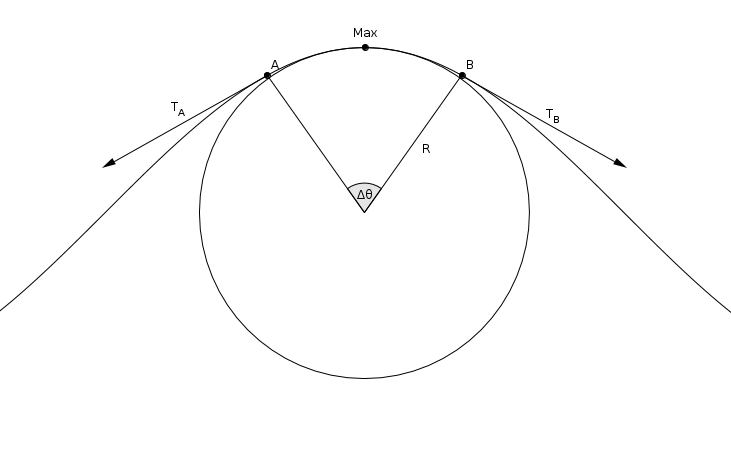
\includegraphics[width=10cm]{imgs/tension.png}
\end{center}
\caption{Force s'appliquant sur le maximum d'une onde dans une corde tendue}
\label{Force s'appliquant sur le maximum d'une onde dans une corde tendue}
\end{figure}
\paragraph{}La longueur du morceau de la corde considéré (entre $A$ et $B$) vaut
\[\Delta l=\Delta \theta R\]
Rappelons aussi que ($T$ est la tension de la corde)
\[\left|\vec{T_A}\right|=\left|\vec{T_B}\right|=T\]
\begin{figure}
\begin{center}
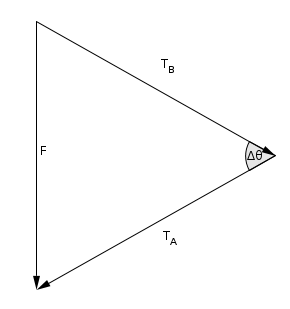
\includegraphics[width=5cm]{imgs/result.png}
\end{center}
\caption{Force résultante des forces de tension}
\label{Force résultante des forces de tension}
\end{figure}
\[\vec{F}=\vec{T_A}+vec{T_B}\]
\[\Rightarrow F=T\Delta\theta\]
\paragraph{}Vu que l'onde est approximée par un cercle $\vec{F}$ est la force centripète et vaut donc
\[F=\Delta m \frac{c^2}{R}\]
\[\Rightarrow T\Delta \theta=\Delta m \frac{c^2}{R}\]
\paragraph{}Vu que $\Delta l=\Delta \theta R$ alors
\[\Rightarrow T\frac{\Delta l}{R}=\Delta m \frac{c^2}{R}\]
\[\Leftrightarrow \Delta m c^2=T\Delta l\]
\[\Leftrightarrow c^2=T\frac{\Delta l}{\Delta m}\]
\[\Leftrightarrow c=\sqrt{\frac{T}{\frac{\Delta m}{\Delta l}}}\]
\[\Leftrightarrow c=\sqrt{\frac{T}{\mu}}\]
\paragraph{}Où $\mu$ est la masse par unité de longueur.
\section{Effet Doppler}
\subsection{Énoncé}
\paragraph{}\textbf{Effet Doppler (source ou observateur mobile par rapport au milieu : quatre cas en tout)}
\subsection{Observateur immobile}
\subsubsection{La source s'éloigne}
\paragraph{}Comme nous pouvons le voir sur la figure la nouvelle longueur d'onde $\lambda'$ est l'ancienne longueur d'onde $\lambda$ plus la distance parcourue par la source entre deux maxima, c'est à dire $vT$. En résumé :
\[\lambda'=\lambda+vT\]
\[\Leftrightarrow cT'=cT+vT=(c+v)T\]
\[\Leftrightarrow \frac{c}{f'}=\frac{c+v}{f}\]
\[\Leftrightarrow \frac{f'}{c}=\frac{f}{c+v}\]
\[\Leftrightarrow f'=\frac{c}{c+v}f\]
\begin{figure}
\begin{center}
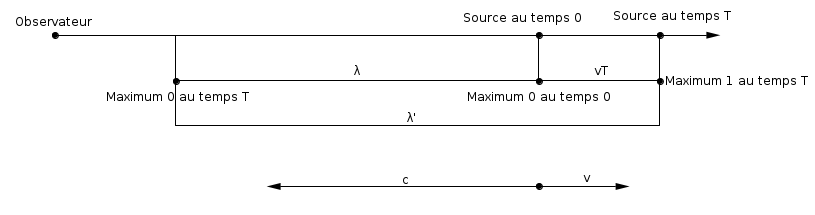
\includegraphics[width=15cm]{imgs/OfSe.png}
\end{center}
\caption{L'effet Doppler : la source s'éloigne d'un observateur fixe par rapport au milieu}
\label{L'effet Doppler : la source s'éloigne d'un observateur fixe par rapport au milieu}
\end{figure}
\subsubsection{La source se rapproche}
\paragraph{}Comme nous pouvons le voir sur la figure la nouvelle longueur d'onde $\lambda'$ est l'ancienne longueur d'onde $\lambda$ moins la distance parcourue par la source entre deux maxima, c'est à dire $vT$. En résumé :
\[\lambda'=\lambda+vT\]
\[\Leftrightarrow cT'=cT-vT=(c-v)T\]
\[\Leftrightarrow \frac{c}{f'}=\frac{c-v}{f}\]
\[\Leftrightarrow \frac{f'}{c}=\frac{f}{c-v}\]
\[\Leftrightarrow f'=\frac{c}{c-v}f\]
\begin{figure}
\begin{center}
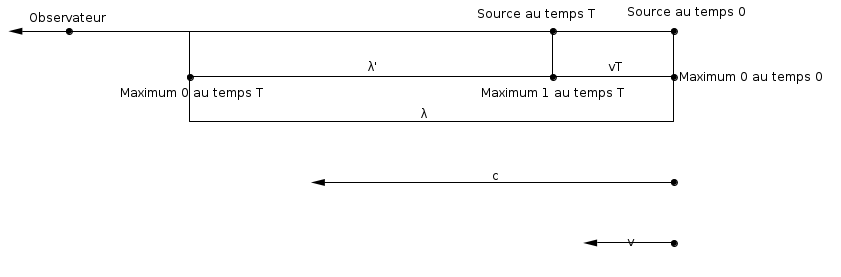
\includegraphics[width=15cm]{imgs/OfSa.png}
\end{center}
\caption{L'effet Doppler : la source se rapproche d'un observateur fixe par rapport au milieu}
\label{L'effet Doppler : la source se rapproche d'un observateur fixe par rapport au milieu}
\end{figure}
\subsection{Source immobile}
\subsubsection{L'observateur s'éloigne}
\paragraph{}Comme nous pouvons le voir sur la figure la nouvelle longueur d'onde $\lambda'$ est l'ancienne longueur d'onde $\lambda$ plus la distance parcourue par la source entre deux maxima, c'est à dire $vT'$. En résumé :
\[\lambda'=\lambda+vT'\]
\[\Leftrightarrow cT'=cT+vT'\]
\[\Leftrightarrow cT'-vT'=cT\]
\[\Leftrightarrow T'(c-v)=cT\]
\[\Leftrightarrow \frac{c-v}{f'}=\frac{c}{f}\]
\[\Leftrightarrow f'=\frac{c-v}{c}f\]
\begin{figure}
\begin{center}
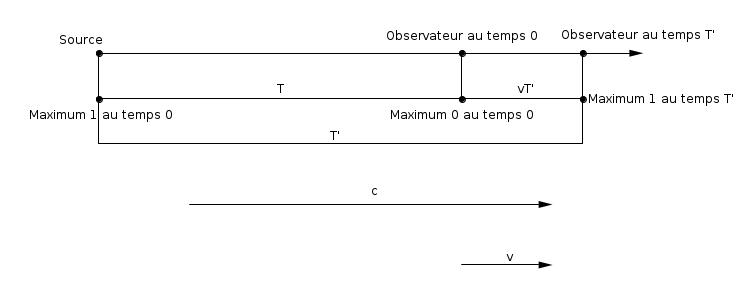
\includegraphics[width=15cm]{imgs/SfOe.png}
\end{center}
\caption{L'effet Doppler : l'observateur s'éloigne de la source fixe par rapport au milieu}
\label{L'effet Doppler : l'observateur s'éloigne de la source fixe par rapport au milieu}
\end{figure}
\subsubsection{L'observateur se rapproche}
\paragraph{}Comme nous pouvons le voir sur la figure la nouvelle longueur d'onde $\lambda'$ est l'ancienne longueur d'onde $\lambda$ moins la distance parcourue par la source entre deux maxima, c'est à dire $vT'$. En résumé :
\[\lambda'=\lambda-vT'\]
\[\Leftrightarrow cT'=cT-vT'\]
\[\Leftrightarrow cT'+vT'=cT\]
\[\Leftrightarrow T'(c+v)=cT\]
\[\Leftrightarrow \frac{c+v}{f'}=\frac{c}{f}\]
\[\Leftrightarrow f'=\frac{c+v}{c}f\]
\begin{figure}
\begin{center}
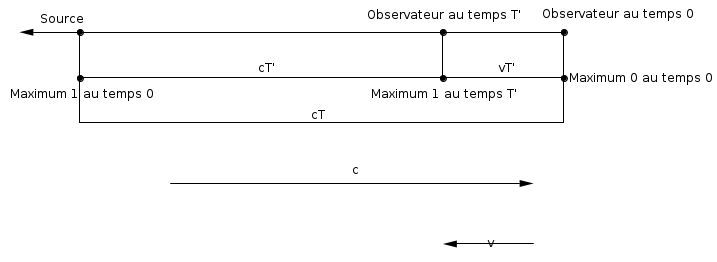
\includegraphics[width=15cm]{imgs/SfOa.png}
\end{center}
\caption{L'effet Doppler : l'observateur se rapproche de la source fixe par rapport au milieu}
\label{L'effet Doppler : l'observateur se rapproche de la source fixe par rapport au milieu}
\end{figure}
\section{Interférences}
\subsection{Énoncé}
\paragraph{}\textbf{figure d'interférence de deux sources ponctuelles synchrones dans le plan : conditions d'interférence constructive et destructive, positions angulaires des nœuds et des ventres.}
\subsection{Interférences de deux sources synchrones dans le plan}
\paragraph{}Soit deux sources $R_1$ et $R_2$ distantes d'une distance $D$. Nous pouvons donc écrire les équations des ondes émises par les deux sources ($r_1$ est la distance entre le point et $R_1$, $r_2$ est la distance entre le point et $R_2$).
\[
\left\{
\begin{array}{r c l}
y_1(t,r_1) &=& Asin\left(2\pi\left(\frac{t}{T}-\frac{r_1}{\lambda}\right)\right)\\
y_2(t,r_2) &=& Asin\left(2\pi\left(\frac{t}{T}-\frac{r_2}{\lambda}\right)\right)\\
\end{array}
\right.
\]
\paragraph{}La résultante $y$ de ces 2 forces est bien entendu leur somme.
\[y(t,r_1,r_2)=y_1(t,r_1)+y_2(t,r_2)\]
\[=Asin\left(2\pi\left(\frac{t}{T}-\frac{r_1}{\lambda}\right)\right)+Asin\left(2\pi\left(\frac{t}{T}-\frac{r_2}{\lambda}\right)\right)\]
\[=2Asin\left(\frac{2\pi\left(\frac{t}{T}-\frac{r_1}{\lambda}\right)+2\pi\left(\frac{t}{T}-\frac{r_2}{\lambda}\right)}{2}\right)cos\left(\frac{2\pi\left(\frac{t}{T}-\frac{r_1}{\lambda}\right)-2\pi\left(\frac{t}{T}-\frac{r_2}{\lambda}\right)}{2}\right)\]
\[=2Acos\left(\pi\left(\frac{r_2-r_1}{\lambda}\right)\right)sin\left(...\right)\]
\paragraph{}Le sinus dépend du temps, nous n'en tiendrons pas compte. Nous calculerons donc uniquement la variation du cosinus.
\paragraph{Nœuds}Le cosinus est à un point d'inflexion lorsqu'il vaut $0$ donc lorsque son paramètre vaut $(2k+1)\frac{\pi}{2} (k \in \mathbb{Z})$. Donc
\[\pi\frac{r_2-r_1}{\lambda}=(2k+1)\frac{\pi}{2} (k \in \mathbb{Z})\]
\[\Leftrightarrow r_2-r_1=(2k+1)\frac{\lambda}{2} (k \in \mathbb{Z})\]
\paragraph{Ventres}Le cosinus est à un extrema lorsqu'il vaut $\pm1$ donc lorsque son paramètre vaut $k\pi (k \in \mathbb{Z})$. Donc
\[\pi\frac{r_2-r_1}{\lambda}=k\pi (k \in \mathbb{Z})\]
\[\Leftrightarrow r_2-r_1=k\lambda (k \in \mathbb{Z})\]
\paragraph{}L'ensemble de points du plan où sont présents les nœuds et les ventres sont donc des hyperboles
\subsection{Rappels sur les hyperboles}
\[r_2-r_1=constante\]
\[=2a\]
\[=2c\text{ }sin\theta\]
\[=Dsin\theta\]
\begin{figure}
\begin{center}
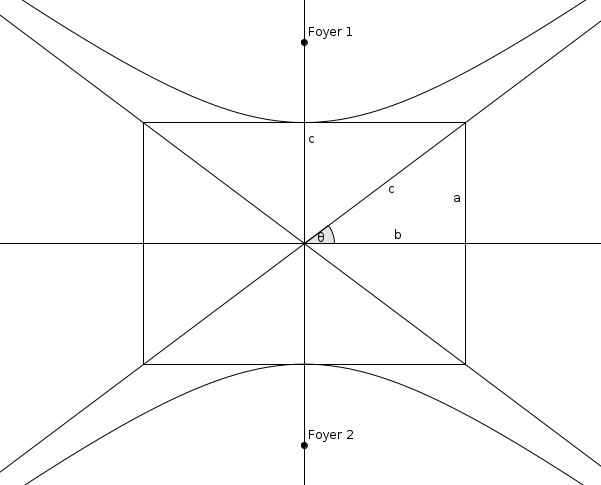
\includegraphics[width=10cm]{imgs/hyperbole.png}
\end{center}
\caption{Rappels sur les hyperboles}
\label{Rappels sur les hyperboles}
\end{figure}
\subsection{Conclusion}
\paragraph{Nœuds}Présence de nœuds si
\[Dsin\theta=(2k+1)\frac{\lambda}{2} (k \in \mathbb{Z})\]
\paragraph{Ventres}Présence de ventres si
\[Dsin\theta=k\lambda (k \in \mathbb{Z})\]
\section{Théorie cinétique des gaz parfaits}
\subsection{Énoncé}
\paragraph{}\textbf{Théorie cinétique des gaz parfaits : modèle fournissant l'énergie cinétique des molécules en fonction de la température. Application aux athmosphères des planètes (y compris le calcul de la vitesse de libération).}
\subsection{Énergie cinétique d'un gaz en fonction de sa température}
\paragraph{}Partons de la loi des gaz parfaits
\[P\mathscr{V}=nRT\]
\[\Leftrightarrow P\mathscr{V}=\frac{nN_ART}{N_A}\]
\[\Leftrightarrow P\mathscr{V}=nN_AkT \text{ où $k$ est la constante de Boltzmann et vaut $\frac{R}{N_A}$.}\]
\[\Leftrightarrow P\mathscr{V}=NkT \text{ où $N$ est le nombre de molécules et vaut bien sûr $N_A\times n$.}\]
\subsubsection{Calcul de la pression exercé par un gaz sur une surface}
Nous pouvons simplifier le mouvement de $N$ molécules d'un gaz de la manière suivante :
\begin{center}
\begin{tabular}{|c|c|c|c|c|c|}
\hline
$\frac{N}{6}$ & $\frac{N}{6}$ & $\frac{N}{6}$ & $\frac{N}{6}$ & $\frac{N}{6}$ & $\frac{N}{6}$ \\
\hline
$\rightarrow$ & $\leftarrow$ & $\uparrow$ & $\downarrow$ & $\otimes$ & $\odot$ \\
\hline
\end{tabular}
\end{center}
\paragraph{Nombre de collisions}Donc le nombre de molécules d'un gaz de volume $\mathscr{V}$ contenant $N$ molécules ayant une vitesse $V$ qui percutent une surface $A$ en un temps $\Delta t$ est :
\[\frac{NVA\Delta t}{6\mathscr{V}}\] 
\paragraph{Force de chaque colission}
Vu que $F=ma$ Alors
\[F=ma=m\frac{\left|\Delta\vec{V}\right|}{\Delta t}\]
\paragraph{}Vu que lors de la collision le sens de la vitesse est inversé, on peut dire qu'il y a une variation de vitesse de $2V$ (elle doit s'arrêter et repartir dans l'autre sens).
\[m\frac{\left|\Delta\vec{V}\right|}{\Delta t}=\frac{2mV}{\Delta t}\]
\paragraph{Force totale}La force totale est le produit de la force de chaque molécule par le nombre de molécule.
\[F_{totale}=\frac{NVA\Delta t}{6\mathscr{V}}\frac{2mV}{\Delta t}=\frac{N}{3\mathscr{V}}V^2mA\]
\paragraph{Pression}À partir de la définition de la pression non savons arrivons à cette formule :
\[P=\frac{F}{A}=\frac{NV^2mA}{3\mathscr{V}A}=\frac{NV^2m}{3\mathscr{V}}\]
\paragraph{}Nous pouvons développer cette formule pour arriver à un résultat intéressant.
\[P=\frac{NV^2m}{3\mathscr{V}}\]
\[\Leftrightarrow P\mathscr{V}=\frac{1}{3}NV^2m=\frac{2}{3}N\left(\frac{1}{2}mV^2\right)\]
\[\Leftrightarrow NkT=\frac{2}{3}N\left(\frac{1}{2}mV^2\right)\]
\[\Leftrightarrow \frac{3}{2}kT=\frac{1}{2}mV^2=E_c\]
\subsection{Calcul de la vitesse de libération}
\paragraph{}Afin de calculer la vitesse de libération, calculons d'abord le travail nécessaire à cette libération.
\[\mathscr{T}=\int_R^{+\infty}\frac{GMm}{r^2}dr=\left[-\frac{GMm}{r}\right]_R^{+\infty}=\frac{GMm}{R}\]
\paragraph{}Pour fournir ce travail, le corps doit posséder une certaine quantité d'énergie. Vu que nous cherchons une vitesse de libération, nous cherchons l'énergie cinétique nécessaire pour accomplir ce travail. Donc
\[E_c=\frac{1}{2}mV_L^2=\frac{GMm}{R}\]
\[\Leftrightarrow V_L=\sqrt{\frac{2GM}{R}}\]
\section{Électromagnétisme}
\subsection{Énoncé}
\paragraph{}\textbf{Loi de Faraday (y compris les conventions de signe). Calcul de l'auto-inductance d'une bobine. Réactance inductive. Déphasage entre l'intensité et la tension.}
\subsection{Rappels}
\paragraph{Champ magnétique}Le champ magnétique à l'intérieur d'un solénoïde, noté $\vec{B}$ vaut
\[\vec{B}=\mu n i\text{ où } \mu=\mu_0\mu_r\]
\paragraph{Flux}Le flux $\Phi$ d'un champ magnétique $\vec{B}$ à l'intérieur d'une surface $A$ vaut
\[\phi=\vec{B}\vec{n}A\]
\paragraph{Loi de Lenz-Faraday}Il apparait une tension électromotrice $\mathscr{E}$ qui vaut
\[\left|\mathscr{E}\right|=\left|\dot{\Phi}\right|=\left|\frac{d\Phi}{dt}\right|\]
\subsection{Formulation mathématique de la loi de Faraday}
\begin{center}\Huge{À finir}\end{center}
\subsection{L'auto-inductance}
\paragraph{}La bobine crée un champ magnétique qui s'oppose à la variation de celui créé par le courant électrique. Si on place la bobine sur du courant alternatif, alors vu que la variation d'intensité est permanente alors, la bobine résiste de manière permanente, cela s'appelle la résistance électromagnétique ou l'impédance.
\[\mathscr{E}(t)=\mathscr{E}_msin(\omega t)\]
\paragraph{}Comment est le flux au sein de la bobine ?
\[\vec{B}_{induit}\vec{n}=\mu n i\]
\[\Leftrightarrow \Phi=\mu niNA\]
\[\Leftrightarrow \mathscr{E}_{induit}(t)=-\dot{\Phi}=-\mu nNA\frac{di}{dt}\]
\[\Rightarrow \mathscr{E}_{induit}(t)=-L\frac{di}{dt}\]
\paragraph{}Où
\[L=\mu nNA=\mu n^2lA\]
\paragraph{}Et l'unité de $L$ est
\[[L]=\frac{V\cdot s}{A}=1\text{ Henry}\]
\paragraph{}Ce nombre $L$ est appelé \textit{coefficient d'auto-inductance}.
\subsection{La réactance inductive}
\begin{figure}
\begin{center}
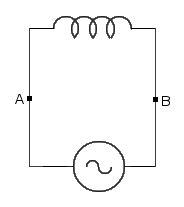
\includegraphics[width=5cm]{imgs/em_1.png}
\end{center}
\caption{La réactance inductive}
\label{La réactance inductive}
\end{figure}
\paragraph{} Tension délivrée par le générateur : $V_A-V_B=\mathscr{E}_msin{\omega t}$
\paragraph{} Tension délivrée par le générateur : $V_B-V_A=-L\frac{di}{dt}$
\[L\frac{di}{dt}=\mathscr{E}_msin(\omega t)\]
\[\Leftrightarrow di=\frac{\mathscr{E}_m}{L}sin(\omega t)dt\]
\[\Leftrightarrow \int di=\int \frac{\mathscr{E}_m}{L}sin(\omega t)dt\]
\[\Leftrightarrow i(t)=-\frac{\mathscr{E}_m}{\omega L}cos(\omega t)dt\]
\paragraph {} $\omega L$ est appelé réactance inductive.
\[=-\frac{\mathscr{E}_m}{\omega L}sin\left(\omega t+ \frac{\pi}{2}\right)dt\]
\[=\frac{\mathscr{E}_m}{\omega L}sin\left(\omega t- \frac{\pi}{2}\right)dt\]
\[\Leftrightarrow i(t)=\frac{\mathscr{E}_m}{\omega L}sin\left(\omega t- \frac{\pi}{2}\right)dt\]
\[\Leftrightarrow \mathscr{E}_m=\omega Li_m \text{ où $i_m$ est l'intensité maximale}\]
\paragraph{}Cette formule rapelle celle du courant continu $U=Ri$
\paragraph{}On remarque que l'intensité est en retard de $\frac{\pi}{2}$ par rapport à la tension.
\end{document}
